\chapter{Драйвер Serial устройства}
\textbf{Цель:} Активация Serial устройства, и написание ПО для работы с ним.

\vspace{5mm}
\textbf{Описание:}Внести правки в device tree для активации Serial контроллера и передачи выводов под его управление. Собрать и протестировать тестовое ПО, которое обеспечивает работу с устройством через Serial интерфейс.

\vspace{5mm}
\textbf{Полезные ссылки:}
\begin{itemize}
	\item \href{https://blog.mbedded.ninja/programming/operating-systems/linux/linux-serial-ports-using-c-cpp/}{Linux Serial Ports Using C/C++}.
	\item \href{https://docs.kernel.org/devicetree/dynamic-resolution-notes.html}{Kernel Doc: Devicetree Dynamic Resolver Notes}
	\item \href{https://www.kernel.org/doc/html/v4.15/driver-api/spi.html}{Kernel Doc: SPI API}	
\end{itemize}

\section{Запуск и подключение к устройству}

\subsection{}Запустите виртуальную машину. Логин и пароль для входа: student / usrstudent.

\subsection{}Подключите по USB плату к ПК. Проверьте, и при необходимости подключите USB устройство FTDI RBM\_C1K5500VK018 к виртуальной машине (меню Device→USB).

\subsection{}Откройте программу gtkterm, и подключитесь к порту /dev/ttyUSB1

\subsection{}Если в окне терминала нет текста, нажмите клавишу Enter на клавиатуре. Вы должны увидеть следующий вывод:
\begin{center}
	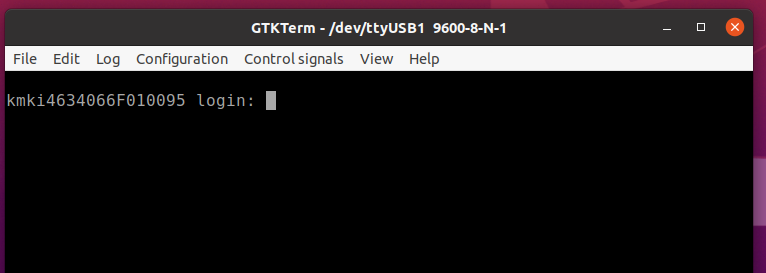
\includegraphics[width=\textwidth]{pic_08}
\end{center}
Вы подключились к консоли устройства. Введите логин root и пароль root.


\section{Подготовка Device Tree Overlay}

\subsection{} Создадим рабочую папку в виртуальной машине для создания device-tree overlay и перейдём в неё 
\begin{lstlisting}[style=bash]
# mkdir $BAGET/lab_07/devtree
# cd $BAGET/lab_07/devtree 
\end{lstlisting}

\subsection{}Создадим новый файл
\begin{lstlisting}[style=bash]
# kate of_serial2.dts
\end{lstlisting}
и запишем в него следующий текст
\begin{lstlisting}[style=stdout]
	/dts-v1/;
	/plugin/;
	/ {
		fragment@0 {
			target-path = "/gpio@1b400200";
			__overlay__ {
				
				serail2_pins {
					phandle = <0x01>;
					uart2_rx {
						function = "uart2_rx";
						groups = "uart2_rx";
					};
					uart2_tx {
						function = "uart2_tx";
						groups = "uart2_tx";
					};
				};
			};
		};
		
		
		fragment@1 { 
			target-path = "/serial@1b511000"; 
			__overlay__ { 
				status = "okay"; 
				pinctrl-names = "default"; 
				pinctrl-0 = <0x01>; 
			}; 
		}; 
		
		
		__local_fixups__ {
			fragment@1 {
				__overlay__ {
					pinctrl-0 = <0x00>;
				};
			};	
		};
	};
\end{lstlisting}

\subsection{}Сохраните изменения Ctrl+S и закройте редактор Ctrl+Q 

\subsection{}Скомпилируем наш фрагмент, для этого выполним следующую команду
\begin{lstlisting}[style=bash]
# dtc --symbol -O dtb -o ./of_serial2.dtb ./of_serial2.dts
\end{lstlisting}

\subsection{}Скопируйте полученный файл на плату
\begin{lstlisting}[style=bash]
# scp ./of_serial2.dtb netuser@192.168.100.200:/home/netuser/
\end{lstlisting}

\subsection{}Перейдите в терминал платы, и переместите файл в папку barebox
\begin{lstlisting}[style=bash]
$ mv /home/netuser/of_serial2.dtb /barebox/
\end{lstlisting}

\subsection{}Откройте скритп barebox.sh для редактирования
\begin{lstlisting}[style=bash]
$ nano /barebox/barebox.sh
\end{lstlisting}
и впишите после строки DTB=k5500vk018\_rbm.dtb следующую строчку
\begin{lstlisting}[style=stdout]
fdt_apply -i $DTB -l of_serial2.dtb -o /dtb && DTB=/dtb
\end{lstlisting}

\subsection{}Сохраните изменения (Ctrl+S, Ctrl+X), и перезагрузите плату (\$ reboot)

\subsection{}После перезагрузки входим в систему (root/root). И выполняем команду
\begin{lstlisting}[style=bash]
$ ls -l /sys/class/tty/ttyS2
\end{lstlisting}
папка должна ссылаться на устройство с адресом активированного нами контроллера, если это не так, значит Вы допустили ошибку в описании дополнения к дереву устройств
\begin{lstlisting}[style=stdout]
/sys/class/tty/ttyS2->../../devices/platform/1b511000.serial/tty/ttyS2
\end{lstlisting}

\section{Тестовое приложение}

\subsection{}Скопируйте исходники в рабочую папку
\begin{lstlisting}[style=bash]
# cp -r $BAGET/support/serial_app $BAGET/lab_07/app
\end{lstlisting}

\subsection{}Перейдём в рабочий каталог, и откроем vscode
\begin{lstlisting}[style=bash]
# cd $BAGET/lab_07/app; code .
\end{lstlisting}

\subsection{}Откроем файл main.c. Как видим тут только две функции. Одна для инициализации UART контроллера, в которой отключаеться вся предобработка отправляемых и принимаемых данных операционной системой, что позволяет нам передавать различные данные через интерфейс без потерь. Так же тут настраивается скорость передачи и приёма. Обратите внимание, потенциально скорость передачи и приёма может быть различной.

В основном коде создаётся два буфера, для приёма и отправки данных. Затем один буфер инициализируется стартовыми значениями, и запускается передача данных. Тут нужно обратить внимание на то, что аппаратный FIFO буфер UART контроллера имеет ограниченный объём, в данном случае 16 бит (считайте значение из файла /sys/class/tty/ttyS2/xmit\_fifo\_size). По этой причине, если Вы не успеете считать 16 бит из приёмного буфера, то всё что будет принято далее, будет потеряно.

\subsection{}Скомпилируйте и отправьте код на целевую платформу
\begin{lstlisting}[style=bash]
# make
# scp ./serapp netuser@192.168.100.200:/home/netuser
\end{lstlisting}

\subsection{}Замкните выводы RX и TX и запустите программу на плате
\begin{lstlisting}[style=bash]
$ /home/netuser/serapp
\end{lstlisting}
Вы должны получить информацию, об успешном завершении. Если нет, то необходимо проверить подключение, и настройки.

\subsection{} Выключите плату, для чего в начале введите команду
\begin{lstlisting}[style=bash]
	$ poweroff
\end{lstlisting}
дождитесь, как появиться надпись
\begin{lstlisting}[style=stdout]
	reboot: System halt
\end{lstlisting}
после чего отключите USB кабель от ПК или платы. 